% ===========================================================================
% Construire des centroïdes
% Traduit et adapté de :
%   https://www.bootstrapworld.org/materials/fall2026/en-us/lessons/measuring-similarity-2/
% Suite de la leçon « Mesurer la similarité »
% Licence : Creative Commons 4.0 Unported (Bootstrap Community)
% ===========================================================================

\documentclass[12pt,a4paper]{article}

% ---------- Packages ----------
\usepackage[utf8]{inputenc}
\usepackage[T1]{fontenc}
\usepackage{libertine}
\usepackage{microtype}
\usepackage[french]{babel}
\usepackage{graphicx}
\usepackage{float}
\usepackage{hyperref}
\usepackage{geometry}
\usepackage{enumitem}
\usepackage{tabularx}
\usepackage{xcolor}
\usepackage{colortbl}
\usepackage[raster]{tcolorbox}
\usepackage{booktabs}
\usepackage{fancyhdr}
\usepackage{titlesec}
\usepackage{amsmath}
\usepackage{amssymb}
\usepackage{listings}

% ---------- Mise en page ----------
\geometry{margin=2.5cm, headheight=15pt, footskip=30pt}
\fancyhf{}
\fancyhead[L]{\textbf{Construire des centroïdes}}
\fancyhead[R]{\thepage}
\fancyfoot[C]{Bootstrap Community — CC BY 4.0}
\renewcommand{\headrulewidth}{0.4pt}
\pagestyle{fancy}

% ---------- Couleurs ----------
\definecolor{bsblue}{RGB}{41,128,185}
\definecolor{bsgreen}{RGB}{39,174,96}
\definecolor{bsorange}{RGB}{230,126,34}
\definecolor{bsgray}{RGB}{149,165,166}
\definecolor{codebg}{RGB}{245,247,250}

% ---------- Styles de sections ----------
\titleformat{\section}[hang]{\Huge\bfseries\color{bsblue}}{}{0pt}{}[\vspace{-0.5em}\rule{\textwidth}{2pt}]
\titleformat{\subsection}[hang]{\Large\bfseries\color{bsblue!80!black}}{}{0pt}{}
\titleformat{\subsubsection}[hang]{\large\bfseries\color{bsgreen!60!black}}{}{0pt}{}

% ---------- Environnements personnalisés ----------
\newtcolorbox{overviewbox}{
  colback=bsblue!5!white, colframe=bsblue!60!white,
  fonttitle=\bfseries, title=Objectif de la section,
  left=1em, right=1em, top=0.5em, bottom=0.5em
}
\newtcolorbox{activitybox}{
  colback=bsgreen!5!white, colframe=bsgreen!60!white,
  fonttitle=\bfseries, title=Activité,
  left=1em, right=1em, top=0.5em, bottom=0.5em
}
\newtcolorbox{thinkbox}{
  colback=bsorange!5!white, colframe=bsorange!60!white,
  fonttitle=\bfseries, title=Réflexion,
  left=1em, right=1em, top=0.5em, bottom=0.5em
}
\newtcolorbox{keypointbox}{
  colback=bsgray!10!white, colframe=bsgray!50!white,
  fonttitle=\bfseries, title=Point clé,
  left=1em, right=1em, top=0.5em, bottom=0.5em
}
\newtcolorbox{instructornotes}{
  colback=yellow!10!white, colframe=yellow!80!black,
  fonttitle=\bfseries, title=Notes pour l'enseignant·e,
  left=1em, right=1em, top=0.5em, bottom=0.5em
}
\newtcolorbox{codebox}{
  colback=codebg, colframe=bsgray!40,
  fonttitle=\bfseries, title=Code Pyret,
  left=1em, right=1em, top=0.5em, bottom=0.5em
}
\newtcolorbox{contractbox}{
  colback=bsblue!3!white, colframe=bsblue!40!white,
  left=1em, right=1em, top=0.6em, bottom=0.6em
}

% ---------- Style listings pour Pyret ----------
\lstdefinelanguage{Pyret}{
  keywords={use,context,url-file,and,or,not,if,else,for,fun,data,sharing,include,import,as,where,let,rec,is,=,true,false,end,Table,String,Number,Boolean,Image,Row,List,Code},
  sensitive=true,
  comment=[l]{\#},
  morestring=[b]",
  morestring=[b]',
}
\lstset{
  language=Pyret,
  basicstyle=\ttfamily\small,
  commentstyle=\color{bsgreen!70!black}\itshape,
  keywordstyle=\color{bsblue}\bfseries,
  stringstyle=\color{bsorange},
  backgroundcolor=\color{codebg},
  frame=single,
  framesep=5pt,
  rulecolor=\color{bsgray!40},
  breaklines=true,
  breakatwhitespace=false,
  showstringspaces=false,
  aboveskip=0.8em,
  belowskip=0.8em,
}

% ---------- Commandes pratiques ----------
\newcommand{\img}[3]{%
  \begin{figure}[H]
    \centering
    \includegraphics[#2]{#1}
    \caption{#3}
    \label{fig:#1}
  \end{figure}
}
\newcommand{\contrat}[1]{%
  \begin{contractbox}
    \ttfamily #1
  \end{contractbox}
}

% ---------- Informations du document ----------
\title{%
  \vspace{-2cm}
  {\Huge\bfseries Construire des centroïdes}\\[0.5em]
  {\large Apprentissage supervisé, recherche par concept et coût humain de l'étiquetage}\\[1em]
  {\normalsize Traduit et adapté depuis \href{https://www.bootstrapworld.org/materials/fall2026/en-us/lessons/measuring-similarity-2/}{Bootstrap World} (Fall 2026)}\\
  {\normalsize Suite de la leçon «~Mesurer la similarité~»}\\[0.5em]
  {\normalsize Licence Creative Commons 4.0 International}
}
\date{}
\author{}

\begin{document}

\maketitle
\thispagestyle{empty}

\vspace{2cm}
\begin{center}
  \textit{Ces supports ont été développés en partie grâce au soutien de la National Science Foundation\\
  (bourses 1042210, 1535276, 1648684, 1738598, 2031479 et 1501927).}
\end{center}

\newpage
\tableofcontents
\newpage

% ===========================================================================
% SECTION 1 : MAIS NOUS N'AVONS ENCORE RIEN APPRIS !
% ===========================================================================
\section[Nous n'avons encore rien appris]{Mais nous n'avons encore rien \emph{appris}~!}

\begin{overviewbox}
  Les élèves considèrent les limites du système de similarité construit dans \emph{Mesurer la similarité}, et apprennent la différence entre apprentissage supervisé et non supervisé.
\end{overviewbox}

% ---------- Launch ----------
\subsection{Lancement}

Dans \emph{Mesurer la similarité}, vous avez appris que les images peuvent être représentées en utilisant différents attributs générés par la machine comme \texttt{WIDTH}, \texttt{LUMINANCE}, \texttt{ENTROPY}, etc. Vous avez aussi appris comment un modèle sac de mots peut transformer une colonne de chaînes en plusieurs colonnes qui comptent le nombre de fois où chaque mot apparaît, nous donnant un compte des pixels \texttt{red}, \texttt{green}, et \texttt{blue}.

Les modèles de similarité sont aussi des \emph{systèmes de recommandation}~! Quand vous demandez à Google de trouver une image correspondant à une photo particulière, vous lui demandez de \emph{recommander} des images similaires.

\img{images/63b290381b2a57b8.png}{width=0.55\textwidth}{Un nuage de points 2D montrant les images tracées sur les axes bleu vs.~vert.}

Vous avez aussi appris que ces attributs générés par la machine peuvent être utilisés pour définir des \emph{espaces}, dans lesquels nous pouvons tracer ces images. Et une fois que nous voyons ces images comme des points dans l'espace, nous pouvons utiliser différentes mesures pour évaluer la similarité.

\begin{thinkbox}
  \begin{itemize}
    \item \textbf{Quelles mesures de similarité avons-nous apprises~?}
    \begin{itemize}
      \item \textbf{Similarité de distance} — mesure la distance euclidienne entre deux points dans un nombre quelconque de dimensions.
      \item \textbf{Similarité d'angle} — mesure l'angle entre les rayons tracés depuis l'origine jusqu'à deux points dans des dimensions de~2 ou plus.
    \end{itemize}
    \item \textbf{Quelles étaient les limites de ces mesures~?}
    \begin{itemize}
      \item La similarité de distance se concentrait sur la distance absolue plutôt que proportionnelle. Notre petit carré rouge était tellement plus petit que le grand que presque toutes les images de montagne avec beaucoup de pixels rouges étaient «~plus proches~», même si ces pixels ne représentaient qu'une petite portion de l'image de montagne.
      \item La similarité d'angle n'est utile qu'en~2~dimensions ou plus, parce que l'angle entre deux points sur la même droite sera toujours zéro.
    \end{itemize}
  \end{itemize}
\end{thinkbox}

% ---------- Investigate ----------
\subsection{Exploration~: les limites de notre système}

Malheureusement, le système que nous avons constrduit jusqu'à présent a deux limites majeures par rapport aux systèmes réels. Commençons par la première~:

\begin{keypointbox}
  \textbf{Nous ne pouvons \emph{rechercher que par document}~:} nous choisissons une image et trouvons des images similaires. Google nous permet de taper un mot comme «~herbe~»~! Spotify nous permet de taper un mot comme «~jazz~», plutôt que de lui demander une chanson spécifique.
\end{keypointbox}

Rappelez-vous, notre système ne \emph{voit} pas réellement la neige sur ces montagnes. Et même s'il le pouvait, il n'a aucune idée de ce que le mot «~neige~» signifie à moins que nous, les humains, ne le lui disions~!

\begin{thinkbox}
  Les ingénieur·es en apprentissage automatique de Netflix, Spotify, et Google ont confronté ces mêmes problèmes~:
  \begin{enumerate}
    \item Les ordinateurs ne savent pas que vous aimez «~Single Ladies~», mais pas «~Lemonade~».
    \item Ils ne savent pas que Jack Black est dans «~Kung-Fu Panda~» \emph{et} «~The Minecraft Movie~».
    \item Ils peuvent nous dire que deux chansons de jazz sont similaires, mais ne peuvent pas juste lancer une station «~jazz~».
    \item \emph{Dans notre exemple}, les ordinateurs savent que nos images de montagnes enneigées sont similaires, mais n'ont aucune idée qu'elles ont toutes de la neige.
  \end{enumerate}

  Alors…~et si \textbf{nous, les humains}, commencions à dire à ces modèles qui est Jack Black, quelles chansons nous aimons, quelles chansons sont du jazz et quelles images ont de la neige~?
\end{thinkbox}

\begin{keypointbox}
  \textbf{Deux types d'apprentissage automatique}

  Il existe plusieurs types d'apprentissage automatique, et jusqu'à présent \textbf{notre système de similarité n'en utilise aucun~!}

  \begin{itemize}
    \item \textbf{Apprentissage non supervisé} — l'ordinateur reçoit un corpus de données et doit trouver des motifs. Il n'y a pas de «~clé de réponses~»~! Nous pourrions demander à l'ordinateur de trouver les \textbf{N} groupes d'images qui sont proches les uns des autres.
    \item \textbf{Apprentissage supervisé} — le corpus a été étiqueté, fournissant une sorte de clé de réponses. L'ordinateur doit trouver des motifs qui associent les entrées aux sorties, en restant aussi proche que possible des bonnes réponses. Nous pourrions maintenant demander à l'ordinateur de trouver des images similaires à celles que nous aimons, ou celles que nous avons étiquetées avec un terme ou un autre.
  \end{itemize}
\end{keypointbox}

% ---------- Synthesize ----------
\subsection{Synthèse}

\begin{thinkbox}
  Quand vous entraîniez des arbres de décision pour identifier l'espèce d'un animal à partir de colonnes comme \texttt{pounds}, \texttt{mammal}, \texttt{swims}, etc., le jeu d'entraînement incluait les «~bonnes réponses~» pour l'espèce de chaque animal.

  \begin{itemize}
    \item \textbf{Était-ce un exemple d'apprentissage supervisé ou non supervisé~?}
    \begin{itemize}
      \item Supervisé.
    \end{itemize}
    \item \textbf{Pourquoi~?}
    \begin{itemize}
      \item Parce que le calcul de similarité n'a \emph{pas utilisé} les étiquettes — même si les données les avaient, nous les avons ignorées.
    \end{itemize}
  \end{itemize}

  Vous avez construit un modèle d'images, incluant des colonnes comme \texttt{ENTROPY}, \texttt{WIDTH}, \texttt{red}, etc.

  \begin{itemize}
    \item \textbf{Était-ce un exemple d'apprentissage supervisé ou non supervisé~?}
    \begin{itemize}
      \item Non supervisé.
    \end{itemize}
    \item \textbf{Pourquoi~?}
    \begin{itemize}
      \item Parce que les données n'avaient aucune étiquette.
    \end{itemize}
    \item \textbf{Dans notre corpus d'images, quelles colonnes pensez-vous être importantes pour l'apprentissage supervisé~?}
    \begin{itemize}
      \item \texttt{LIKES}, \texttt{DISLIKES}, et \texttt{TAGS}.
    \end{itemize}
  \end{itemize}
\end{thinkbox}

\newpage

% ===========================================================================
% SECTION 2 : QUE L'APPRENTISSAGE COMMENCE !
% ===========================================================================
\section{Que l'apprentissage commence~!}

\begin{overviewbox}
  Les élèves ajoutent des étiquettes pour les likes, dislikes, et tags à leur corpus d'images, et utilisent des fonctions auxiliaires pour voir comment cet étiquetage élargit la puissance de la recherche d'images.
\end{overviewbox}

% ---------- Launch ----------
\subsection{Lancement~: trouver le centre}

\begin{activitybox}
  Ouvrez le \textbf{fichier Images Similaires} (\texttt{Images\allowbreak-Similaires\allowbreak-Starter.arr}) et cliquez sur «~Run~», puis évaluez \texttt{mountains} dans la Zone d'Interactions.

  \begin{itemize}
    \item \textbf{Quelles images ont de la \textbf{neige} visible~?}
    \begin{itemize}
      \item \texttt{"snow1"} et \texttt{"snow2"}.
    \end{itemize}
    \item \textbf{Quelles images ont de l'\textbf{herbe} visible~?}
    \begin{itemize}
      \item \texttt{"grass"} et \texttt{"grass\allowbreak-sun"} (et peut-être un peu de \texttt{"sun1"}).
    \end{itemize}
    \item \textbf{Quelles images ont un \textbf{soleil} visible (soit un coucher soit un lever)~?}
    \begin{itemize}
      \item \texttt{"sun1"}, \texttt{"grass\allowbreak-sun"}, \texttt{"sun2"}, et \texttt{"sunset"}.
    \end{itemize}
  \end{itemize}
\end{activitybox}

\img{images/63b290381b2a57b8.png}{width=0.5\textwidth}{Nuage de points 2D sur les axes bleu vs.~vert.}

\begin{thinkbox}
  \textbf{Quand nous cherchons une image qui a un soleil visible, nous voulons une image qui soit similaire à ce que les images de soleil \emph{ont en commun}.}

  \textbf{Comment pouvons-nous trouver la «~soleil-itude~» d'une image~?}
\end{thinkbox}

\img{images/edf6f26564ae88c9.png}{width=0.5\textwidth}{Nuage de points 2D sur les axes bleu vs.~vert. Deux des images sont reliées par une ligne fine, avec le centre de la ligne marqué d'une croix.}

\begin{keypointbox}
  \textbf{Le centroïde}

  Si chaque image de notre corpus est un point dans l'espace, alors le terrain commun est littéralement un point \emph{au milieu}. Nous avons un ensemble d'images contenant le soleil, et nous voulons trouver le centre.

  Dans notre Espace Bleu-Vert à 2~dimensions, par exemple, le point à mi-chemin entre \texttt{"grass\allowbreak-sun"} et \texttt{"sun2"} définit une sorte de «~soleil-itude~»~!
\end{keypointbox}

\begin{instructornotes}
  (Vous rappelez-vous avoir appris la moyenne, la médiane, et le mode~? En apprentissage automatique, il existe des algorithmes pour trouver des groupes de points dans l'espace qui s'appellent littéralement \emph{k-means}, \emph{k-medians}, et \emph{k-modes} clustering~! \emph{Les mesures de tendance centrale sont une partie critique de l'apprentissage automatique moderne.})
\end{instructornotes}

\begin{thinkbox}
  \begin{itemize}
    \item \textbf{Nous avons \textbf{trois} images où le soleil est visible. Comment pouvons-nous trouver le milieu de ces trois~?}
    \begin{itemize}
      \item C'est le milieu d'un triangle~!
    \end{itemize}
    \item \textbf{Pouvons-nous trouver le milieu d'une forme 3D~?}
    \begin{itemize}
      \item Oui~!
    \end{itemize}
  \end{itemize}
\end{thinkbox}

\begin{activitybox}
  Complétez la première section de \emph{Apprentissage supervisé}.
\end{activitybox}

\begin{keypointbox}
  \textbf{Le centroïde en 1, 2, et 3~dimensions}

  Si vous avez plus d'une dimension, les mêmes maths s'appliquent~: calculez le centroïde pour chaque colonne séparément. Pouvez-vous obtenir un meilleur résultat pour les images ensoleillées en enseignant à Pyret à quoi ressemble la «~soleil-itude~» pour deux de nos images~?

  Pour tout ensemble de points (dans un nombre quelconque de dimensions~!), le «~milieu~» est le \textbf{centroïde}.

  \begin{center}
  \begin{tabular}{c c c}
    \textbf{En 1~dimension…} & \textbf{En 2~dimensions…} & \textbf{En 3~dimensions…} \\
    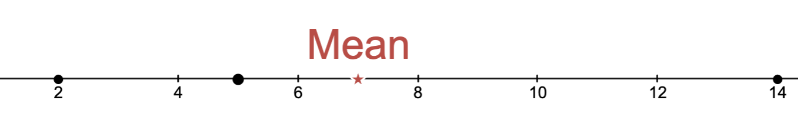
\includegraphics[width=0.28\textwidth]{images/acd9781ba7f1f852.png} &
    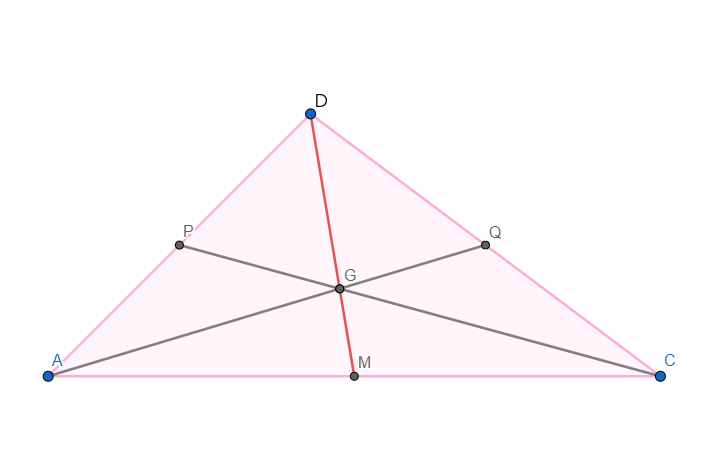
\includegraphics[width=0.28\textwidth]{images/b61f7d69cf00791e.png} &
    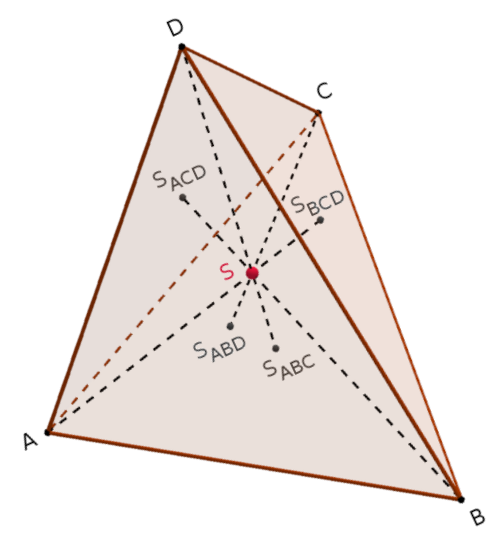
\includegraphics[width=0.28\textwidth]{images/ebc59617cd4ea367.png} \\
  \end{tabular}
  \end{center}

  \begin{center}
  \small\emph{De gauche à droite~: droite numérique avec points à 2, 5, et~14, et le centroïde étiqueté comme la moyenne~; triangle avec des bissectrices convergeant vers le centroïde~; tétraèdre avec son centroïde.}
  \end{center}
\end{keypointbox}

% ---------- Investigate ----------
\subsection{Exploration~: recherche par concept et recommandation}

\img{images/ebc59617cd4ea367.png}{width=0.3\textwidth}{Tétraèdre avec son centroïde.}

\begin{thinkbox}
  \begin{itemize}
    \item \textbf{Même sans aucun véritable \emph{apprentissage}, notre mesure \texttt{angle-similarity} faisait du bon travail en recommandant des images similaires quand on lui donnait une image herbeuse ou enneigée. Pourquoi a-t-elle eu du mal à trouver des images avec le soleil~?}
    \begin{itemize}
      \item L'image de coucher de soleil est \emph{vraiment} différente des autres. Chaque fois que nous cherchons par l'\texttt{ID} des autres images (\texttt{"sun1"}, \texttt{"grass-sun"}, ou \texttt{"sun2"}), nous obtenons d'autres recommandations avant \texttt{"sunset"}.
    \end{itemize}
  \end{itemize}
\end{thinkbox}

\begin{keypointbox}
  \textbf{Rappelez-vous le plus grand problème de notre système sans apprentissage~:}

  \begin{itemize}
    \item Nous ne recommandons des correspondances que sur la base d'un \emph{seul document}~: nous ne pouvons pas trouver des images, des chansons, ou quoi que ce soit d'autre sur la base d'une \emph{collection} de documents aimés ou non aimés.
  \end{itemize}

  \textbf{Comment notre implémentation du centroïde peut-elle résoudre ce problème aussi~?}

  Construire des centroïdes est l'endroit où nous \textbf{commençons à généraliser entre les lignes}, parce que maintenant nous pouvons accéder au pouvoir de l'information étiquetée par les humains pour raisonner sur des \emph{groupes}. Au lieu de regarder une image avec de l'herbe, nous pouvons maintenant regarder plusieurs images herbeuses et parler de \emph{ce qu'elles ont en commun~: «~l'herbe-itude~»}.

  Et nous pouvons utiliser cela pour résoudre \textbf{les deux} limites de notre système non supervisé~!
  \begin{itemize}
    \item Nous pouvons trouver un centroïde pour toutes les images étiquetées «~sun~», et l'utiliser pour trouver des images \emph{non} étiquetées qui sont proches de la «~soleil-itude~». Sans centroïdes, nous sommes coincés à comparer des images à \textbf{une photo avec un soleil}.
    \item Nous pouvons trouver un centroïde pour toutes les images \emph{aimées} ou \emph{non aimées}, puis recommander des images non étiquetées proches de la «~aimé-itude~» et éloignées de la «~non-aimé-itude~». Sans centroïdes, nous sommes coincés à comparer des images à \textbf{une seule image aimée}.
  \end{itemize}
\end{keypointbox}

\begin{keypointbox}
  \textbf{Les trois étapes sont les mêmes dans chaque cas~:}
  \begin{enumerate}
    \item Trouver tous les documents étiquetés (aimés, non aimés, étiquetés, etc.).
    \item Construire un centroïde.
    \item Trouver les documents non étiquetés qui sont similaires au centroïde en utilisant les colonnes pertinentes.
  \end{enumerate}
\end{keypointbox}

\begin{activitybox}
  Nous avons fourni deux fonctions qui font exactement cela, en utilisant toutes les colonnes disponibles dans la table.

  Complétez la deuxième section de \emph{Apprentissage supervisé}.
\end{activitybox}

\begin{thinkbox}
  \begin{itemize}
    \item \textbf{Pourquoi la construction d'un centroïde à partir de \texttt{"grass-sun"} et \texttt{"sun2"} nous a-t-elle aidés à améliorer la recommandation~?}
    \begin{itemize}
      \item Parce que le centroïde était «~plus proche~» de toutes les images de soleil qu'aucune d'entre elles ne l'était de toutes les autres.
    \end{itemize}
  \end{itemize}
\end{thinkbox}

\subsubsection{Recommander à partir d'une collection}

\begin{keypointbox}
  Maintenant un système de recommandation se résume à~:
  \begin{itemize}
    \item Calculer les centroïdes pour les documents aimés et non aimés.
    \item Calculer les similarités entre chaque document et les deux centroïdes.
    \item La force de la recommandation est une simple équation~:
  \end{itemize}

  \[
  \text{force} = \text{similarité\,aux\,aimés} - \text{similarité\,aux\,non\,aimés}
  \]

  Nous avons créé une fonction auxiliaire qui fait exactement cela, étant donné une table et une liste de colonnes~:

  \contrat{\# recommend :: (Table t) -> Table}

  Le résultat est une table de tous vos documents, par ordre décroissant de force de recommandation (la plus forte en premier).
\end{keypointbox}

\subsubsection{Recherche par mot-clé}

\begin{keypointbox}
  La recherche d'images par mot se résume à~:
  \begin{itemize}
    \item Trouver tous les documents étiquetés avec ce mot, et calculer leur centroïde.
    \item Calculer la similarité de tous les documents à ce centroïde.
    \item La précision de la correspondance est la similarité elle-même.
  \end{itemize}

  Nous avons créé une fonction auxiliaire qui fait exactement cela, étant donné une table et une liste de colonnes~:

  \contrat{\# search-by-tag :: (Table t, List<String> tags) -> Table}

  Le résultat est une table de tous vos documents, par ordre décroissant de similarité au centroïde des documents qui correspondent à votre étiquette.
\end{keypointbox}

\begin{activitybox}
  Complétez la dernière section de \emph{Apprentissage supervisé}.

  Pouvez-vous faire la différence entre apprentissage supervisé et non supervisé dans le monde réel~? Pouvez-vous faire la différence entre les modèles supervisés qui utilisent des classificateurs, la régression, ou la similarité~?

  Complétez \emph{Supervisé ou non supervisé~?}.
\end{activitybox}

\begin{instructornotes}
  Pour plus de pratique, demandez aux élèves de compléter \emph{Supervisé ou non supervisé~? (Suite)}. Après qu'ils ont terminé, faites la révision en désignant un côté de la classe comme «~supervisé~» et l'autre comme «~non supervisé~», et demandez aux élèves de se déplacer d'un côté ou de l'autre selon leur confiance.
\end{instructornotes}

\subsubsection{Et pour d'autres catégories~?}

\begin{thinkbox}
  Nous avons exploré la construction d'un modèle pour comparer des images sur la base d'un ensemble d'attributs. Pensons aux attributs à partir desquels nous pourrions construire des modèles pour d'autres catégories de choses qui ne sont pas des images~!

  \begin{itemize}
    \item \textbf{Si nous voulions comparer des sports d'équipe, nous pourrions mesurer des attributs comme le \textbf{score gagnant médian} ou la \textbf{probabilité de blessure grave}. Quels autres attributs quantitatifs pouvez-vous imaginer pour comparer des sports d'équipe~?}
    \begin{itemize}
      \item Quantité de contact physique, nombre de joueur·euses par équipe, durée de jeu, pourcentage de temps où le jeu est arrêté…
    \end{itemize}
    \item \textbf{Quels attributs quantitatifs pourrions-nous utiliser pour comparer des films~?}
    \begin{itemize}
      \item Niveau de peur, durée, niveau de violence, niveau d'humour, pourcentage du film qui est animé, nombre d'effets spéciaux…
    \end{itemize}
    \item \textbf{Quels attributs quantitatifs pourrions-nous utiliser pour comparer des styles de pantalons~?}
    \begin{itemize}
      \item Largeur des jambes, hauteur de taille, nombre de poches, longueur des jambes…
    \end{itemize}
  \end{itemize}
\end{thinkbox}

\begin{activitybox}
  Avec votre voisin·e, complétez \emph{Comparer des desserts}.
\end{activitybox}

\begin{thinkbox}
  \begin{itemize}
    \item \textbf{Quels autres attributs avez-vous trouvés pour comparer des desserts~?}
    \begin{itemize}
      \item Douceur, salinité, crémosité, calories…
    \end{itemize}
    \item \textbf{Quelles idées avez-vous eues sur la façon dont nous pourrions \textbf{mesurer} la similarité entre deux exemples~?}
    \item \textbf{L'un ou l'autre des nuages de points que vous avez faits soutenait-il l'idée que les desserts que vous avez marqués comme favori et deuxième favori étaient similaires~?}
    \item \textbf{Pourrions-nous utiliser nos mesures de similarité d'angle ou de distance pour recommander des desserts~?}
    \item \textbf{Quels sont quelques exemples de systèmes de recommandation dans le monde réel, et quels attributs pensons-nous qu'ils pourraient utiliser~?}
  \end{itemize}
\end{thinkbox}

% ---------- Synthesize ----------
\subsection{Synthèse~: le coût humain de l'apprentissage supervisé}

\begin{thinkbox}
  Vous vous souvenez peut-être des étapes de l'apprentissage supervisé d'une leçon précédente~:
  \begin{itemize}
    \item Des données étiquetées par des humains sont enregistrées, démontrant les connaissances à apprendre.
    \item L'algorithme d'apprentissage automatique trouve une \textbf{fonction} qui généralise (espérons-le bien~!) de ces données vers de nouvelles données jamais vues.
    \item La fonction est appliquée à de nouvelles données.
  \end{itemize}
\end{thinkbox}

\img{images/bb2026a7194ff4df.png}{width=0.4\textwidth}{ALVINN / Navlab, une ambulance militaire reconvertie en voiture autonome.}

\begin{thinkbox}
  Une voiture autonome reçoit une table d'entrées (données de divers capteurs), chaque ligne étiquetée avec la façon dont un humain a tourné le volant. Puis elle trouve une fonction qui prédit l'angle du volant à partir de nouvelles entrées, et utilise la fonction en l'appliquant à de nouvelles routes.

  \begin{itemize}
    \item \textbf{Dans notre exemple de recherche d'images, quelles sont les données étiquetées par des humains pour l'ordinateur~?}
    \begin{itemize}
      \item La table d'entrée étiquetée avec des likes ou des dislikes, ou des mots.
    \end{itemize}
    \item \textbf{Quel algorithme est utilisé pour trouver des images~?}
    \begin{itemize}
      \item Une sorte de mesure d'angle pour la similarité, suivie d'un tri.
    \end{itemize}
    \item \textbf{Où est la généralisation~?}
    \begin{itemize}
      \item Une nouvelle image non étiquetée ajoutée à la base de données est toujours comparée aux centroïdes pré-calculés.
    \end{itemize}
  \end{itemize}
\end{thinkbox}

\begin{thinkbox}
  \begin{itemize}
    \item \textbf{Quand vous dites à Spotify que vous aimez une chanson, quels calculs se produisent sur les serveurs de Spotify~?}
    \begin{itemize}
      \item Avec une nouvelle liste de «~chansons aimées~», Spotify recalcule mon centroïde «~aimé~».
    \end{itemize}
    \item \textbf{Quand vous demandez à Spotify de créer une station Jazz, quels calculs se produisent~?}
    \begin{itemize}
      \item Spotify calcule le centroïde pour toutes les chansons \textbf{déjà étiquetées} «~jazz~», puis renvoie celles-ci aux côtés des chansons qui sont similaires au centroïde.
    \end{itemize}
    \item \textbf{Quand vous cherchez «~soleil~» sur Google Images, quels calculs se produisent~?}
    \begin{itemize}
      \item Google calcule le centroïde pour toutes les images \textbf{déjà étiquetées} «~soleil~», puis renvoie celles-ci aux côtés des images similaires au centroïde.
    \end{itemize}
    \item \textbf{Comment Google sait-il filtrer les images offensantes de violence extrême~?}
    \begin{itemize}
      \item Google calcule le centroïde pour toutes les images \textbf{déjà étiquetées} comme extrêmement violentes, puis filtre les images qui sont similaires au centroïde.
    \end{itemize}
  \end{itemize}
\end{thinkbox}

\begin{keypointbox}
  \textbf{Le coût humain de l'étiquetage}

  \begin{itemize}
    \item \textbf{Avec des dizaines de millions d'images dans la base de Google, combien ont dû être étiquetées par des humains pour que les résultats soient précis~?}
    \begin{itemize}
      \item Des centaines~? Des milliers~?
    \end{itemize}
    \item \textbf{Quels humains étiquettent ces images~?}
    \begin{itemize}
      \item \textbf{Nous~!} Qu'est-ce qu'un CAPTCHA à votre avis~?
      \item Des humains sont payés pour le faire.
    \end{itemize}
  \end{itemize}

  L'apprentissage supervisé est en grande partie ce qui fait que les modèles d'apprentissage automatique semblent «~comprendre~» les humains. Quand nous tapons une phrase sur Google Images, on dirait que le moteur de recherche a \emph{compris} ce que nous voulions~! Mais en réalité, c'est un autre algorithme piloté par les données qui triture des océans de données étiquetées et non étiquetées.

  Mais cela a un coût~: \textbf{quelqu'un doit étiqueter des millions d'images~!}
\end{keypointbox}

\img{images/2d91cbf686b35167.png}{width=0.4\textwidth}{Un CAPTCHA demandant à l'utilisateur·trice d'identifier quelles images contiennent des bus.}

\begin{keypointbox}
  Dans certains cas, c'est \textbf{nous}, en cliquant sur des images de bus pour prouver que nous sommes humains. Ces images sont de vraies images d'une base de données où la similarité n'était pas assez forte pour être certain qu'elles sont ou ne sont pas un bus. En nous demandant de les étiqueter, nous aidons à entraîner l'algorithme.

  Mais dans d'autres cas, ce sont des sous-traitant·es payé·es, souvent dans des pays en développement où les entreprises technologiques peuvent les payer quelques euros (ou centimes~!) par jour pour regarder des dizaines de milliers d'images et les étiqueter.

  Les systèmes de similarité sont aussi utilisés pour filtrer les images violentes et offensantes, en les comparant à un corpus d'images étiquetées comme violentes et offensantes. Mais \emph{quelqu'un} a dû regarder ces images pour commencer~! Voir des dizaines de milliers d'images violentes ou offensantes peut avoir de graves impacts sur la santé mentale.

  Nous pensons rarement au coût humain de l'entraînement des modèles d'apprentissage automatique que nous utilisons tous les jours. Quand nous demandons à Google de trouver des images similaires ou à Spotify de recommander de la musique à partir de nos likes et dislikes, nous pensons rarement au rôle important que l'apprentissage supervisé joue pour que tout cela fonctionne…~et aux humains responsables de fournir cette supervision.
\end{keypointbox}

\begin{instructornotes}
  Si vous travaillez avec des élèves plus âgé·es et plus matures, nous suggérons de leur faire lire et discuter \href{https://www.thebrink.me/the-ghosts-in-the-machine-inside-ai-hidden-human-trauma/}{\emph{The Ghosts in the Machine~: Inside AI's Hidden Human Trauma}} de Matt Hussey.
\end{instructornotes}

\newpage

% ===========================================================================
% ANNEXES
% ===========================================================================
\section*{Annexe A~: Supervisé vs.\ non supervisé}

\begin{center}
\begin{tabularx}{\textwidth}{l X X}
  \toprule
  \textbf{Concept} & \textbf{Apprentissage non supervisé} & \textbf{Apprentissage supervisé} \\
  \midrule
  Données       & Sans étiquette                          & Étiquetées par des humains \\
  Clé de réponses & Aucune                                & Fournie (colonne \texttt{LIKED}, \texttt{DISLIKED}, \texttt{TAGS}, etc.) \\
  Objectif      & Trouver des motifs (clusters)           & Apprendre une fonction entrée $\to$ sortie \\
  Exemples      & \texttt{distance-similarity}, \texttt{angle-similarity} sur données brutes & Arbres de décision, régression linéaire, centroïdes d'images étiquetées \\
  généralisation & Entre les lignes (clusters de points)  & Au-delà des données d'entraînement (prédictions sur de nouvelles entrées) \\
  \bottomrule
\end{tabularx}
\end{center}

\section*{Annexe B~: Fichiers du projet}

\begin{center}
\begin{tabularx}{\textwidth}{l X}
  \toprule
  \textbf{Fichier} & \textbf{Description} \\
  \midrule
  \texttt{Images\allowbreak-Similaires\allowbreak-Starter.arr} & Fichier de démarrage Pyret (inchangé par rapport à la leçon précédente). Fournit \texttt{recommend}, \texttt{search-by-tag}, \texttt{distance-similarity}, \texttt{angle-similarity}, etc. via \texttt{ai-library.arr}. \\
  \texttt{construire-centroides.tex} & Document de cours (ce fichier) \\
  \texttt{images/} & 8~images~: nuages de points, centroïdes 1D/2D/3D, ALVINN/Navlab, CAPTCHA \\
  \bottomrule
\end{tabularx}
\end{center}

\vspace{1em}
\textbf{À noter~:} cette leçon utilise \emph{le même} fichier de démarrage que la leçon précédente (\emph{Mesurer la similarité}). Aucune modification du code n'est nécessaire~: les fonctions \texttt{recommend} et \texttt{search-by-tag} sont fournies par \texttt{ai-library.arr} et utilisent les colonnes \texttt{LIKED}, \texttt{DISLIKED}, et \texttt{TAGS} déjà définies dans le starter. Les noms de colonnes restent en anglais car ils sont codés en dur dans la bibliothèque.

\section*{À propos de ces supports}

Ces supports ont été développés en partie grâce au soutien de la \emph{National Science Foundation} (bourses 1042210, 1535276, 1648684, 1738598, 2031479 et 1501927).

\begin{center}
  \textbf{Bootstrap} par la Communauté Bootstrap est sous licence Creative Commons 4.0 Unported.\\
  Cette licence n'accorde pas la permission d'organiser des formations ou du développement professionnel.\\[1em]
  \textit{Traduction et adaptation française réalisées en juillet 2026.}\\
  \textit{Source originale~: \url{https://www.bootstrapworld.org/materials/fall2026/en-us/lessons/measuring-similarity-2/}}
\end{center}

\end{document}